\section{结果}

\subsection{语汇存在，但密度不等于思想深度}

完全匹配首先排除了凭印象写作。“王阳明”在该版本中为0命中，故正文统一使用命中538次的“王守仁”；“格物致知”为0命中，也不作为原书引语。可保留的思想史语汇呈明显层级：“心学”38次、“理学”29次、“书院”20次、“讲学”17次、“良知”16次、“知行合一”12次，而更具体的“致良知”只有2次。该分布说明叙事乐于反复使用人物与学派标签，却较少持续展开专门命题。

两处逐字证据限定了我们的解释。原书明确写“这件工具的名字叫做‘知行合一’”，随后又把它解释为可实际运用的处事方法；在徐阶师承段则写“此学即所谓‘致良知’之心学，传我此学者，名王守仁”。前者把哲学压缩成行动能力，后者把学说压缩成可沿人物关系传递的知识。它们支持“行动化”与“师承化”的叙事判断，却不能替代对原始哲学文本的概念分析。

\subsection{师承是显著通道，但不是主要边界}

\begin{figure}[!t]
\centering
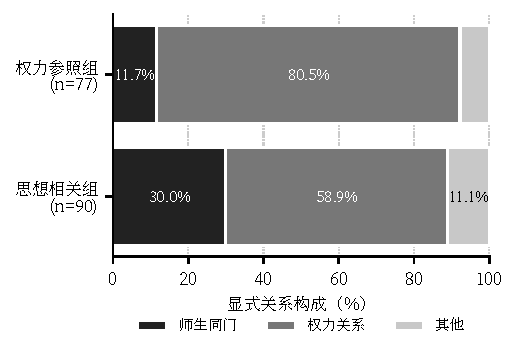
\includegraphics[width=\columnwidth]{figures/fig_ideology_1.pdf}
\caption{思想相关组与权力参照组的显式关系构成。思想组的师生同门占比更高，但权力关系仍占过半；类别为互斥编码。}
\label{fig:ideology-composition}
\end{figure}

全图“师生同门”只有63条，占2.7\%；但在10名思想相关人物的90条显式关系中，该类有27条、占30.0\%，高出全图基线。权力参照组有77条显式关系，其中师生同门9条、占11.7\%。恢复自动推导边后，两组相应占比降为18.2\%与7.3\%，方向不变。由此可见，师承确是思想人物的区别性连接方式，而不是全图普遍现象。

但“区别性”不等于“自治”。思想组的君臣从属、政治攻讦、敌对冲突、同盟友党合计53条，占58.9\%，仍高于师承边；参照组为62条，占80.5\%。思想传播网络并非悬浮在朝廷之外，而是以较高的师承比例嵌入一个仍由权力关系占多数的网络。图\ref{fig:ideology-composition}因此不支持“思想先自由生长、随后才被权力碰触”的简单二阶段模型。

\begin{table}[!t]
\caption{六个锚点的显式关系构成}
\label{tab:ideology-anchors}
\centering
\begin{tabular}{@{}lrrrr@{}}
\toprule
人物 & 度数 & 显式边 & 师生同门 & 权力关系 \\
\midrule
王守仁 & 50 & 36 & 8（22.2\%） & 21（58.3\%）\\
徐阶 & 67 & 42 & 17（40.5\%） & 24（57.1\%）\\
顾宪成 & 18 & 7 & 1（14.3\%） & 4（57.1\%）\\
高攀龙 & 11 & 1 & 1（100.0\%） & 0（0.0\%）\\
张居正 & 66 & 45 & 8（17.8\%） & 35（77.8\%）\\
严嵩 & 59 & 33 & 1（3.0\%） & 28（84.8\%）\\
\bottomrule
\end{tabular}
\end{table}

锚点差异进一步阻止我们把“思想型”本质化。王守仁度数50，显式边中师生同门与政治攻讦各8条；徐阶度数67，17条师生同门使其传播占比达到40.5\%，但其24条权力关系仍占57.1\%。张居正度数66，师生同门也有8条，说明权力人物同样通过门生网络运作。真正形成对照的是严嵩：33条显式边中敌对冲突14条、政治攻讦7条，而师生同门仅1条。可计算的结论不是“思想人物没有权力”，而是思想相关人物把师承通道带进了权力网络。

\subsection{时间序列：形成、间隔与制度冲突}

\begin{figure}[!t]
\centering
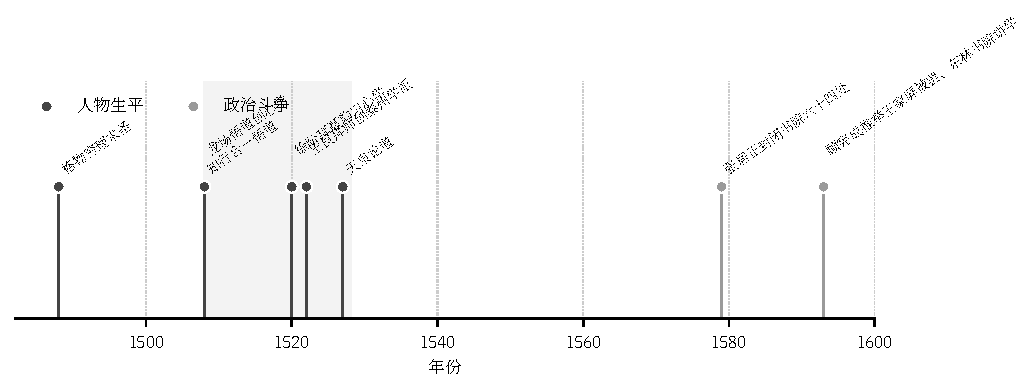
\includegraphics[width=\columnwidth]{figures/fig_ideology_2.pdf}
\caption{8件思想相关事件的年份分布。1508--1528窗口集中5件形成与传播事件，1579与1593出现两件被编码为政治斗争的书院事件。}
\label{fig:ideology-timeline}
\end{figure}

8件事件中，1488年“格物穷理”构成前史；1508年同时出现“龙场悟道创心学”和“知行合一悟道”；1520年徐阶拜聂豹习心学，1522年王艮拜师创泰州学派，1527年天泉论道。因而1508--1528窗口集中了5件，占全部8件的62.5\%。1529--1578窗口没有符合窄筛选规则的事件，这一空白只能解释为本书编码的叙事间隔，不能解释为思想活动中止。

晚期两个节点改变了类别。原书逐字写“万历七年（1579），张居正下令，关闭天下书院，共计六十四处”；结构化事件将其编码为政治斗争。1593年的顾宪成罢官与东林书院讲学同样被编码为政治斗争。8件思想事件中，人物生平6件、占75.0\%，政治斗争2件、占25.0\%。从形成到制度冲突的转折真实存在于叙事编码中，但“收编”不是直接字段：关闭书院、讲学入党争只是可观察替代量。

\subsection{反例与边界情形}

高攀龙显式关系仅1条，恰为师生同门，导致100.0\%这一比例极不稳定；顾宪成显式关系7条且七类各1条，同样不宜单独外推。另一方面，何心隐到王守仁的再传弟子关系被编码为“亲属”，暴露类别噪声。组层面的90条显式边比单人百分比稳健，但仍受抽取规则约束。本文因此把个体表作为诊断，不把它当作精确人物排名。
